\documentclass{ximera}

% These macros are automatically generated from the "macros"
% XML element.  Make permanent edits there.
%
% History
%   2004/01/01  Initiated for FCLA, evolved from there
%   2006/09/17  Converted  _, ^  to \sb, \sp for TeX4ht
%   2014/02/01  Updated for MathBook XML projects
%               Obsolete in FCLA: \codeindent, \computerfont, \define
%               Change: MathJax wants \lt, so replaced by \lteval
%   2014/02/22  New: \orderof, \reals, \per
%   2015/08/16  Incorporated into MathBook XML version of FCLA
%
%%%%%%%%%%%%%%%%%%%%%
%
%     Conveniences
%
%%%%%%%%%%%%%%%%%%%%%
%
%  Order of (asymptotically limit of fraction is 1)
%  Usage: \orderof{some function}
%
\newcommand{\orderof}[1]{\sim #1}
%
%  Integers
%  Usage:  \Z
\newcommand{\Z}{\mathbb{Z}}
%
%  Real numbers, as set of scalars
%  Usage:  \reals
\newcommand{\reals}{\mathbb{R}}
%
%  n-space over real field
%  Usage: \complex{integer-dimension}
\newcommand{\real}[1]{\mathbb{R}^{#1}}
%
%  Complex numbers, as set of scalars
%  Usage:  \complexes
\newcommand{\complexes}{\mathbb{C}}
%
%  n-space over complex field
%  Usage: \complex{integer-dimension}
\newcommand{\complex}[1]{\mathbb{C}^{#1}}
%
%  Complex conjugation (scalar, vector, matrix)
%  Usage: \conjugate{object}
\newcommand{\conjugate}[1]{\overline{#1}}
%
%  Complex number modulus
%  Usage: \modulus{a+bi}
%  Presumes math mode
\newcommand{\modulus}[1]{\left\lvert#1\right\rvert}
%
%  Zero vector
%  Usage: \zerovector
\newcommand{\zerovector}{\vect{0}}
%
%  Zero matrix
%  Usage: \zeromatrix, use a subscript when size is important
\newcommand{\zeromatrix}{\mathcal{O}}
%
%  Inner product (brackets, not quadratic form)
%  Usage: \innerproduct{a-vector}{a-vector}
\newcommand{\innerproduct}[2]{\left\langle#1,\,#2\right\rangle}
%
%  Norm of a vector
%  Usage: \norm{a-vector}
\newcommand{\norm}[1]{\left\lVert#1\right\rVert}
%
%  Dimension
%  Usage: \dimension{vector-space-letter}
\newcommand{\dimension}[1]{\dim\left(#1\right)}
%
%  Nullity
%  Usage: \nullity{matrix-or-lintrans-letter}
\newcommand{\nullity}[1]{n\left(#1\right)}
%
%  Rank
%  Usage: \rank{matrix-or-lintrans-letter}
\newcommand{\rank}[1]{r\left(#1\right)}
%
%  Direct sum
%  Usage: \ds between a couple of subspaces
%
\newcommand{\ds}{\oplus}
%
%  Determinant of a matrix (functional)
%  Usage: \detname{A}
\newcommand{\detname}[1]{\det\left(#1\right)}
%
%  Determinant of a matrix (vertical bars)
%  Usage: \detbars{A}
\newcommand{\detbars}[1]{\left\lvert#1\right\rvert}
%
%  Trace of a Matrix
%  Usage: \trace{matrix name}
\newcommand{\trace}[1]{t\left(#1\right)}
%
%  Square Root of a Matrix
%  Usage: \sr{a-matrix}
\newcommand{\sr}[1]{#1^{1/2}}
%
%%%%%%%%%%%%%%%%%%%%%
%
%     Subspace Constructions
%
%%%%%%%%%%%%%%%%%%%%%
%
%  Span of a set of vectors
%  \span and \sp are used by TeX for other things
%  Usage: \spn{set-of-vectors}
\newcommand{\spn}[1]{\left\langle#1\right\rangle}
%
%  Null space of a matrix
%  Usage:  \nsp{A}
\newcommand{\nsp}[1]{\mathcal{N}\!\left(#1\right)}
%
%  Column space of a matrix
%  Usage:  \csp{A}
\newcommand{\csp}[1]{\mathcal{C}\!\left(#1\right)}
%
%  Row space of a matrix
%  Usage:  \rsp{A}
\newcommand{\rsp}[1]{\mathcal{R}\!\left(#1\right)}
%
%  Left null space of a matrix
%  Usage:  \lns{A}
\newcommand{\lns}[1]{\mathcal{L}\!\left(#1\right)}
%
%  Orthogonal complement of a vector space
%  Avoiding TeX's \perp
%  Usage:  \per{A}
\newcommand{\per}[1]{#1^\perp}
%
%%%%%%%%%%%%%%%%%%%%%
%
%     Systems of Equations
%
%%%%%%%%%%%%%%%%%%%%%
%
%  In-line form of an augmented matrix for a system of equations
%  Usage: \augmented{coefficient-matrix}{constant-vector}
\newcommand{\augmented}[2]{\left\lbrack\left.#1\,\right\rvert\,#2\right\rbrack}
%
%  Notation for a linear system before introducing matrix multiplication
%  Usage: \linearsystem{coefficient-matrix}{constant-vector}
\newcommand{\linearsystem}[2]{\mathcal{LS}\!\left(#1,\,#2\right)}
%
%  Notation for a homogenous system before introducing matrix multiplication
%  Usage: \homosystem{coefficient-matrix}
\newcommand{\homosystem}[1]{\linearsystem{#1}{\zerovector}}
%
%%%%%%%%%%%%%%%%%%%%%
%
%     Row Operations, Echelon Form
%
%%%%%%%%%%%%%%%%%%%%%
%
% Row operations on matrices
%
% Three commands to shorten up descriptions of gaussian elimination
%
% Usage: \rowopswap{row-i}{row-j}
% Usage: \rowopmult{scalar}{row-i}
% Usage: \rowopadd{scalar}{row-multiplied}{row-added-to}
\newcommand{\rowopswap}[2]{R_{#1}\leftrightarrow R_{#2}}
\newcommand{\rowopmult}[2]{#1R_{#2}}
\newcommand{\rowopadd}[3]{#1R_{#2}+R_{#3}}
%
% Mark leading 1's in echelon form with fbox
% Usage: \leading{a-1-usually}
\newcommand{\leading}[1]{\fbox{#1}}
%
%  Row-reduce arrow
%  Usage:  \rref inbetween a matrix and its reduced row-echelon form
\newcommand{\rref}{\xrightarrow{\text{RREF}}}
%
%  Elementary Matrices
%  Usage: \elemswap{subscript}{subscript}
%  Usage: \elemmult{scalar}{subscript}
%  Usage: \elemadd{scalar}{subscript-mult}{subscript-target}
%
\newcommand{\elemswap}[2]{E_{#1,#2}}
\newcommand{\elemmult}[2]{E_{#2}\left(#1\right)}
\newcommand{\elemadd}[3]{E_{#2,#3}\left(#1\right)}
%
%%%%%%%%%%%%%%%%%%%%%
%
%     2-D Constructions (Lists, Vectors, Matrices)
%
%%%%%%%%%%%%%%%%%%%%%
%
%  A list of scalars of generic length
%  Usage:  \scalarlist{scalar letter}{terminal subscript}
\newcommand{\scalarlist}[2]{{#1}_{1},\,{#1}_{2},\,{#1}_{3},\,\ldots,\,{#1}_{#2}}
%
%  Vector styling, bold (or use wiggles, arrows, whatever)
%  Subscripts go outside this construction
%  Usage: \vect{a symbol to use as a vector}
%  Have to already be in math mode
%
\newcommand{\vect}[1]{\mathbf{#1}}
%
%  A column vector
%  Usage: \colvector{list-delimited-by-\\}
%
\newcommand{\colvector}[1]{\begin{bmatrix}#1\end{bmatrix}}
%
%  A generic vector with components
%  Usage: \vectorcomponents{component-letter}{final-subscript}
\newcommand{\vectorcomponents}[2]{\colvector{#1_{1}\\#1_{2}\\#1_{3}\\\vdots\\#1_{#2}}}
%
%  A list of vectors of generic length
%  Usage:  \vectorlist{vector letter}{terminal subscript}
\newcommand{\vectorlist}[2]{\vect{#1}_{1},\,\vect{#1}_{2},\,\vect{#1}_{3},\,\ldots,\,\vect{#1}_{#2}}
%
%  Vector entries, entry i of vector v
%  (vector-expession still needs \vect, etc.)
%  Usage:  \vectorentry{vector-expression}{single-subscript}
\newcommand{\vectorentry}[2]{\left\lbrack#1\right\rbrack_{#2}}
%
%  Matrix entries, entry i,j of matrix A
%  Usage:  \matrixentry{matrix-expression}{paired-subscripts}
%
\newcommand{\matrixentry}[2]{\left\lbrack#1\right\rbrack_{#2}}
%
%  A generic linear combination
%  Usage:  \lincombo{scalar letter}{vector letter}{terminal subscript}
\newcommand{\lincombo}[3]{#1_{1}\vect{#2}_{1}+#1_{2}\vect{#2}_{2}+#1_{3}\vect{#2}_{3}+\cdots +#1_{#3}\vect{#2}_{#3}}
%
%  Matrix, column by column, as vectors
%  Usage:  \matrixcolumns{matrix letter}{terminal subscript}
\newcommand{\matrixcolumns}[2]{\left\lbrack\vect{#1}_{1}|\vect{#1}_{2}|\vect{#1}_{3}|\ldots|\vect{#1}_{#2}\right\rbrack}
%
%%%%%%%%%%%%%%%%%%%%%
%
%     Special Matrices
%
%%%%%%%%%%%%%%%%%%%%%
%
%  Transpose of a matrix
%  Usage:  \transpose{A}
\newcommand{\transpose}[1]{#1^{t}}
%
%  Inverse of a matrix
%  Usage:  \inverse{A}
\newcommand{\inverse}[1]{#1^{-1}}
%
%  Submatrix (for minors, determinants)
%  Usage: \submatrix{matrix-name}{delete-row}{delete-col}
\newcommand{\submatrix}[3]{#1\left(#2|#3\right)}
%
%  Adjoint of a matrix (twice)
%  This macro is a convenience to call \transpose and \conjugate properly
%  It shouldn't need to be modified (or mathematical meanings will change)
%  Usage:  \adj{A}
\newcommand{\adj}[1]{\transpose{\left(\conjugate{#1}\right)}}
%
%  This macro controls the symbol used for the adjoint
%  It can be edited to taste
%  Usage:  \adjoint{A}
\newcommand{\adjoint}[1]{#1^\ast}
%
%%%%%%%%%%%%%%%%%%%%%
%
%     Sets
%
%%%%%%%%%%%%%%%%%%%%%
%
%  A convenience for simple sets
%  Usage:  \set{list of element}
\newcommand{\set}[1]{\left\{#1\right\}}
%
%  Sets with vertical bar, "such that", sized for objects, not condition
%  Usage:  \setparts{objects}{condition}
%
%%\newcommand{\setparts}[2]{\left\{ #1\mid#2\right\}}
%%\newcommand{\setparts}[2]{\left\{\left. #1\right\rvert#2\right\}}
\newcommand{\setparts}[2]{\left\lbrace#1\,\middle|\,#2\right\rbrace}
%
%  Set Cardinality
%  Usage:  \card{a-set-letter}
\newcommand{\card}[1]{\left\lvert#1\right\rvert}
%
%  Set Union
%  Use \cup
%
%  Set Intersection
%  Use \cap
%
%  Set Complement
%  Usage:  \setcomplement{a-set-letter}
\newcommand{\setcomplement}[1]{\overline{#1}}
%
%%%%%%%%%%%%%%%%%%%%%
%
%     Eigenvalues and Eigenspaces
%
%%%%%%%%%%%%%%%%%%%%%
%
%  Characteristic polynomial
%  Usage: \charpoly{matrix-letter}{variable-letter}
\newcommand{\charpoly}[2]{p_{#1}\left(#2\right)}
%
%  Eigenspace
%  Usage: \eigenspace{matrix-letter}{eigenvalue-letter}
\newcommand{\eigenspace}[2]{\mathcal{E}_{#1}\left(#2\right)}
%
%  2013/10/03 Including ampersands is problematic here, 
%  think about fixes later
%  2014/02/22 Limited testing, seems &amp; is fine for HTML and LaTeX
%  2016-07-20 only employed in Archetypes, MBX has gather/align override
%  Eigensystem (presumes wrapped in an mrow within md)
%  Usage: \eigensystem{matrixletter}{eigenvalue}{list of basis vectors}
\newcommand{\eigensystem}[3]{\lambda&amp;=#2&amp;\eigenspace{#1}{#2}&amp;=\spn{\set{#3}}} 
%
%  Generalized Eigenspace
%  Usage: \geneigenspace{lin-trans-letter}{eigenvalue-letter}
\newcommand{\geneigenspace}[2]{\mathcal{G}_{#1}\left(#2\right)}
%
%  Algebraic multiplicty
%  Usage: \algmult{matrix-letter}{eigenvalue-letter}
\newcommand{\algmult}[2]{\alpha_{#1}\left(#2\right)}
%
%  Geometric multiplicty
%  Usage: \geomult{matrix-letter}{eigenvalue-letter}
\newcommand{\geomult}[2]{\gamma_{#1}\left(#2\right)}
%
%  Index (of eigenvalue)
%  Usage: \indx{matrix-letter}{eigenvalue-letter}
\newcommand{\indx}[2]{\iota_{#1}\left(#2\right)}
%
%%%%%%%%%%%%%%%%%%%%%
%
%     Linear Transformations
%
%%%%%%%%%%%%%%%%%%%%%
%
%  MathJax defines \lt to ease XML confusion
%
%  Linear transformation definition
%  Usage: \ltdefn{name-letter}{domain}{range}
\newcommand{\ltdefn}[3]{#1\colon #2\rightarrow#3}
%
%  Linear transformation evaluation
%  Usage: \lteval{name-letter}{input}
%  Replaces old \lt desired by MathJax
\newcommand{\lteval}[2]{#1\left(#2\right)}
%
% Linear transformation inverse
%  Usage: \ltinverse{name-letter}
\newcommand{\ltinverse}[1]{#1^{-1}}
%
%  Linear transformation restriction
%  Usage: \restrict{name-letter}{subspace-letter}
\newcommand{\restrict}[2]{{#1}|_{#2}}
%
%  Linear transformation preimage
%  Usage: \preimage{name-letter}{codomain-element}
\newcommand{\preimage}[2]{#1^{-1}\left(#2\right)}
%
%  Range of a linear transformation
%  TeX uses \range for something else
%  Usage:  \rng{T}
\newcommand{\rng}[1]{\mathcal{R}\!\left(#1\right)}
%
%  Kernel of a linear transformation
%  TeX uses \ker to do something different
%  Usage:  \krn{T}
\newcommand{\krn}[1]{\mathcal{K}\!\left(#1\right)}
%
%  Linear transformation composition
%  Usage: \compose{function-name}{function-name}
\newcommand{\compose}[2]{{#1}\circ{#2}}
%
%  Vector space of linear transformations
%  Usage: \vslt{domains}{codomains}
%  Presumes math mode
\newcommand{\vslt}[2]{\mathcal{LT}\left(#1,\,#2\right)}
%
%%%%%%%%%%%%%%%%%%%%%
%
%     Vector and Matrix Representations
%
%%%%%%%%%%%%%%%%%%%%%
%
%  Isomorphism symbol
%  Usage: \isomorphic
\newcommand{\isomorphic}{\cong}
%
%  Similarity
%  Usage: \similar{inner-matrix}{outer-invertible-matrix}
%  Rearranging this will not "fix" all desired changes throughout
%
\newcommand{\similar}[2]{\inverse{#2}#1#2}
%
%  Vector representation function name
%  Usage: \vectrepname{basis-letter}
\newcommand{\vectrepname}[1]{\rho_{#1}}
%
%  Vector representation output
%  Usage: \vectrep{basis-letter}{input}
\newcommand{\vectrep}[2]{\lteval{\vectrepname{#1}}{#2}}
%
%  Vector representation inverse function name
%  (Added later, not used consistently in FCLA)
%  Usage: \vectrepinvname{basis-letter}
\newcommand{\vectrepinvname}[1]{\ltinverse{\vectrepname{#1}}}
%
%  Vector representation inverse output
%  Usage: \vectrepinv{basis-letter}{input}
\newcommand{\vectrepinv}[2]{\lteval{\ltinverse{\vectrepname{#1}}}{#2}}
%
%  Matrix representation
%  Usage: \matrixrep{transformation-letter}{domain-basis-letter}{codomain-basis-letter}
\newcommand{\matrixrep}[3]{M^{#1}_{#2,#3}}
%
%  Matrix representation column-by-colum
%  2016-07-20 only employed once?
%  Usage: \matrixrepcolumns{transformation-letter}{codomain-basis-letter}{codomain-basis-vector-letter}{final-index}
\newcommand{\matrixrepcolumns}[4]{\left\lbrack \left.\vectrep{#2}{\lteval{#1}{\vect{#3}_{1}}}\right|\left.\vectrep{#2}{\lteval{#1}{\vect{#3}_{2}}}\right|\left.\vectrep{#2}{\lteval{#1}{\vect{#3}_{3}}}\right|\ldots\left|\vectrep{#2}{\lteval{#1}{\vect{#3}_{#4}}}\right.\right\rbrack}
%
%  Change of basis matrix
%  Usage: \cbm{domain-basis-letter}{codomain-basis-letter}
\newcommand{\cbm}[2]{C_{#1,#2}}
%
%%%%%%%%%%%%%%%%%%%%%
%
%     Canonical Forms
%
%%%%%%%%%%%%%%%%%%%%%
%
%  Jordan blocks
%  Usage: \jordan{size}{diagonal-element}
\newcommand{\jordan}[2]{J_{#1}\left(#2\right)}
%
%%%%%%%%%%%%%%%%%%%%%
%
%     Hadamard Matrices
%     Contributed by Elizabeth Million
%
%%%%%%%%%%%%%%%%%%%%%
%
%  Hadamard Product
%  Usage: \hadamard{a-matrix}{a-matrix}
\newcommand{\hadamard}[2]{#1\circ #2}
%
%  Hadamard identity matrix
%  Usage: \hadamardidentity{paired-subscripts-size-of-matrix}
\newcommand{\hadamardidentity}[1]{J_{#1}}
%
%  Hadamard inverse matrix
%  Usage: \hadamardinverse{matrix-expression}
\newcommand{\hadamardinverse}[1]{\widehat{#1}}


\title{Examples of Injective Linear Transformations}

\begin{document}
\begin{abstract}
  We consider examples of injective functions, and examples that are not injective.
\end{abstract}
\maketitle

It is perhaps most instructive to examine a linear transformation that is not injective first.

\begin{example}[Not injective]

Consider the linear transformation
\[
\ltdefn{T}{\complex{5}}{\complex{5}},\quad
\lteval{T}{\colvector{x_1\\x_2\\x_3\\x_4\\x_5}}=
\colvector{-2 x_1 + 3 x_2 + 3 x_3 - 6 x_4 + 3 x_5\\
-16 x_1 + 9 x_2 + 12 x_3 - 28 x_4 + 28 x_5\\
-19 x_1 + 7 x_2 + 14 x_3 - 32 x_4 + 37 x_5\\
-21 x_1 + 9 x_2 + 15 x_3 - 35 x_4 + 39 x_5\\
-9 x_1 + 5 x_2 + 7 x_3 - 16 x_4 + 16 x_5}
\]

Notice that for
\begin{align*}
\vect{x}&=\colvector{1\\3\\-1\\2\\4}&
\vect{y}&=\colvector{4\\7\\0\\5\\7}
\end{align*}
so we have
\end{align*}
\lteval{T}{\colvector{1\\3\\-1\\2\\4}}&=\colvector{4\\55\\72\\77\\31}&
\lteval{T}{\colvector{4\\7\\0\\5\\7}}&=\colvector{4\\55\\72\\77\\31}
\end{align*}

So we have two vectors from the domain, $\vect{x}\neq\vect{y}$, yet $\lteval{T}{\vect{x}}=\lteval{T}{\vect{y}}$, in violation of \ref{definition:ILT}.  This is another example where you should not concern yourself with how $\vect{x}$ and $\vect{y}$ were selected, as this will be explained shortly.  However, do understand \textit{why} these two vectors provide enough evidence to conclude that $T$ is not injective.

\end{example}

Here is a cartoon of a non-injective linear transformation.  Notice that the central feature of this cartoon is that $\lteval{T}{\vect{u}}=\vect{v}=\lteval{T}{\vect{w}}$.  Even though this happens again with some unnamed vectors, it only takes one occurrence to destroy the possibility of injectivity.  Note also that the two vectors displayed in the bottom of $V$ have no bearing, either way, on the injectivity of $T$.
\begin{image}
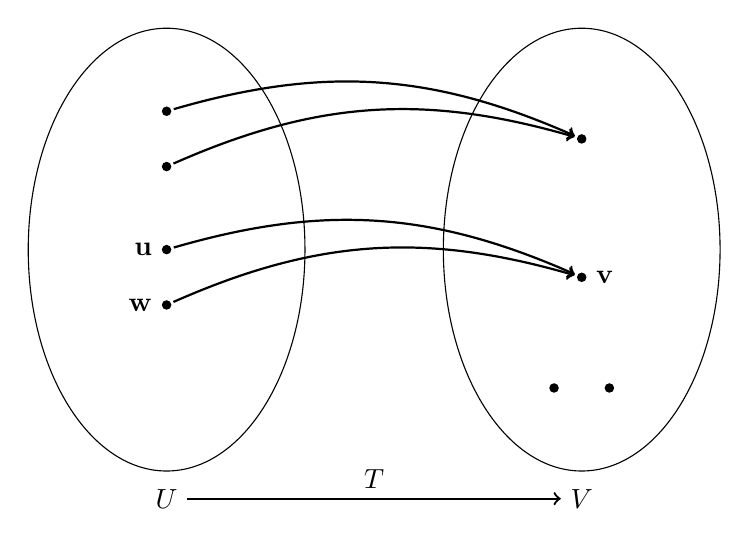
\begin{tikzpicture}
\tikzset{ltvect/.style={shape=circle, minimum size=0.30em, inner sep=0pt, draw, fill=black}}
\tikzset{ltedge/.style={->, bend left=20, thick, shorten <=0.1em, shorten >=0.1em}}
<!--  base generic picture -->
\draw ( 5em, 8em) circle [x radius=5em, y radius=8em, thick];
\draw (20em, 8em) circle [x radius=5em, y radius=8em, thick];
\node (U) at ( 5em, -1em) {$U$};
\node (V) at (20em, -1em) {$V$};
\draw[->, thick, draw] (U) to node[auto] {$T$} (V);
<!--  inputs -->
\node (u1) [ltvect]                         at (5em, 13em) {};
\node (u2) [ltvect]                         at (5em, 11em) {};
\node (u)  [ltvect, label=left:$\vect{u}$]  at (5em,  8em) {};
\node (w)  [ltvect, label=left:$\vect{w}$]  at (5em,  6em) {};
<!--  outputs -->
\node (v1) [ltvect]                         at (20em, 12em) {};
\node (v)  [ltvect, label=right:$\vect{v}$] at (20em,  7em) {};
\node (v2) [ltvect]                         at (19em,  3em) {};
\node (v3) [ltvect]                         at (21em,  3em) {};
<!--  associations -->
\draw[ltedge] (u1) to (v1);
\draw[ltedge] (u2) to (v1);
\draw[ltedge] (u)  to (v);
\draw[ltedge] (w)  to (v);
\end{tikzpicture}
\end{image}

To show that a linear transformation is not injective, it is enough to find a single pair of inputs that get sent to the identical output.  However, to show that a linear transformation is injective we must establish that this coincidence of outputs \textit{never} occurs.  Here is an example that shows how to establish this.

\begin{example}[Injective]

Consider the linear transformation
\[
\ltdefn{R}{\complex{5}}{\complex{5}},\quad
\lteval{R}{\colvector{x_1\\x_2\\x_3\\x_4\\x_5}}=
\colvector{-65 x_1 + 128 x_2 + 10 x_3 - 262 x_4 + 40 x_5\\
36 x_1 - 73 x_2 - x_3 + 151 x_4 - 16 x_5\\
-44 x_1 + 88 x_2 + 5 x_3 - 180 x_4 + 24 x_5\\
34 x_1 - 68 x_2 - 3 x_3 + 140 x_4 - 18 x_5\\
12 x_1 - 24 x_2 - x_3 + 49 x_4 - 5 x_5}
\]

To establish this is injective we must begin with the assumption that $\lteval{R}{\vect{x}}=\lteval{R}{\vect{y}}$ and somehow arrive at the conclusion that $\vect{x}=\vect{y}$.  Here we go,
\begin{align*}
\colvector{0\\0\\0\\0\\0}
&=\lteval{R}{\vect{x}}-\lteval{R}{\vect{y}}\\
&=\lteval{R}{\colvector{x_1\\x_2\\x_3\\x_4\\x_5}}-\lteval{R}{\colvector{y_1\\y_2\\y_3\\y_4\\y_5}}\\
&=
\colvector{-65 x_1 + 128 x_2 + 10 x_3 - 262 x_4 + 40 x_5\\
36 x_1 - 73 x_2 - x_3 + 151 x_4 - 16 x_5\\
-44 x_1 + 88 x_2 + 5 x_3 - 180 x_4 + 24 x_5\\
34 x_1 - 68 x_2 - 3 x_3 + 140 x_4 - 18 x_5\\
12 x_1 - 24 x_2 - x_3 + 49 x_4 - 5 x_5}\\
&\quad\quad-
\colvector{-65 y_1 + 128 y_2 + 10 y_3 - 262 y_4 + 40 y_5\\
36 y_1 - 73 y_2 - y_3 + 151 y_4 - 16 y_5\\
-44 y_1 + 88 y_2 + 5 y_3 - 180 y_4 + 24 y_5\\
34 y_1 - 68 y_2 - 3 y_3 + 140 y_4 - 18 y_5\\
12 y_1 - 24 y_2 - y_3 + 49 y_4 - 5 y_5}\\
&=
\colvector{-65 (x_1-y_1) + 128 (x_2-y_2) + 10 (x_3-y_3) - 262 (x_4-y_4) + 40 (x_5-y_5)\\
36 (x_1-y_1) - 73 (x_2-y_2) - (x_3-y_3) + 151 (x_4-y_4) - 16 (x_5-y_5)\\
-44 (x_1-y_1) + 88 (x_2-y_2) + 5 (x_3-y_3) - 180 (x_4-y_4) + 24 (x_5-y_5)\\
34 (x_1-y_1) - 68 (x_2-y_2) - 3 (x_3-y_3) + 140 (x_4-y_4) - 18 (x_5-y_5)\\
12 (x_1-y_1) - 24 (x_2-y_2) - (x_3-y_3) + 49 (x_4-y_4) - 5 (x_5-y_5)}\\
&=
\begin{bmatrix}
-65&128&10&-262&40\\
36&-73&-1&151&-16\\
-44&88&5&-180&24\\
34&-68&-3&140&-18\\
12&-24&-1&49&-5
\end{bmatrix}
\colvector{x_1-y_1\\x_2-y_2\\x_3-y_3\\x_4-y_4\\x_5-y_5}
\end{align*}


Now we recognize that we have a homogeneous system of 5 equations in 5 variables (the terms $x_i-y_i$ are the variables), so we row-reduce the coefficient matrix to
\[
\begin{bmatrix}
\leading{1}&0&0&0&0\\
0&\leading{1}&0&0&0\\
0&0&\leading{1}&0&0\\
0&0&0&\leading{1}&0\\
0&0&0&0&\leading{1}
\end{bmatrix}
\]




So the only solution is the trivial solution
\begin{align*}
x_1-y_1&=0&x_2-y_2&=0&x_3-y_3&=0&x_4-y_4&=0&x_5-y_5&=0
\end{align*}
and we conclude that indeed $\vect{x}=\vect{y}$.  By \ref{definition:ILT}, $T$ is injective.

\end{example}

Here is the cartoon for an injective linear transformation.  It is meant to suggest that we never have two inputs associated with a single output.  Again, the two lonely vectors at the bottom of $V$ have no bearing either way on the injectivity of $T$.
\begin{image}
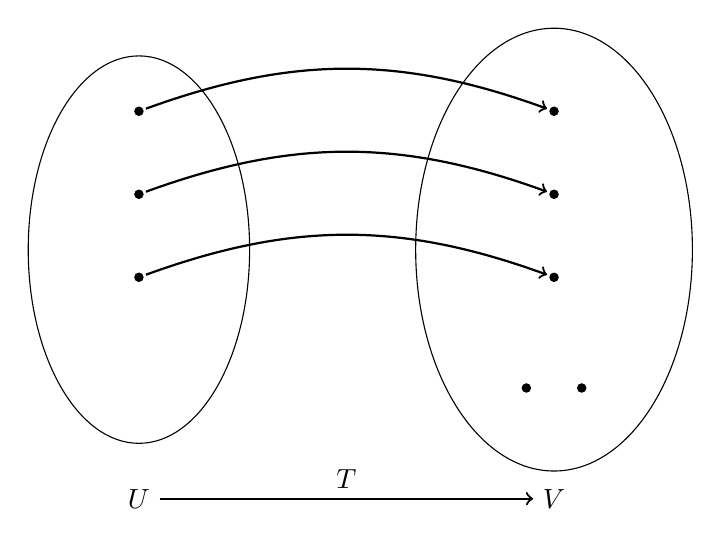
\begin{tikzpicture}
\tikzset{ltvect/.style={shape=circle, minimum size=0.30em, inner sep=0pt, draw, fill=black}}
\tikzset{ltedge/.style={->, bend left=20, thick, shorten <=0.1em, shorten >=0.1em}}
<!--  base generic picture -->
\draw ( 5em, 8em) circle [x radius=4em, y radius=7em, thick];
\draw (20em, 8em) circle [x radius=5em, y radius=8em, thick];
\node (U) at ( 5em, -1em) {$U$};
\node (V) at (20em, -1em) {$V$};
\draw[->, thick, draw] (U) to node[auto] {$T$} (V);
<!--  inputs -->
\node (u1) [ltvect] at (5em, 13em) {};
\node (u2) [ltvect] at (5em, 10em) {};
\node (u3) [ltvect] at (5em,  7em) {};
<!--  outputs -->
\node (v1) [ltvect] at (20em, 13em) {};
\node (v2) [ltvect] at (20em, 10em) {};
\node (v3) [ltvect] at (20em,  7em) {};
\node (v4) [ltvect] at (19em,  3em) {};
\node (v5) [ltvect] at (21em,  3em) {};
<!--  associations -->
\draw[ltedge] (u1) to (v1);
\draw[ltedge] (u2) to (v2);
\draw[ltedge] (u3) to (v3);
\end{tikzpicture}
\end{image}

Let us now examine an example between abstract vector spaces.

\begin{example}

Consider the linear transformation
\[
\ltdefn{T}{P_3}{M_{22}},\quad\lteval{T}{a+bx+cx^2+dx^3}=
\begin{bmatrix}
a+b & a-2c\\
d & b-d
\end{bmatrix}
\]

Suppose that two polynomial inputs yield the same output matrix,
\[
\lteval{T}{a_1+b_1x+c_1x^2+d_1x^3}=\lteval{T}{a_2+b_2x+c_2x^2+d_2x^3}
\]

Then
\begin{align*}
\zeromatrix
&=\begin{bmatrix}
0&0\\0&0
\end{bmatrix}\\
&=\lteval{T}{a_1+b_1x+c_1x^2+d_1x^3}-\lteval{T}{a_2+b_2x+c_2x^2+d_2x^3}&&\text{Hypothesis}\\
&=\lteval{T}{(a_1+b_1x+c_1x^2+d_1x^3)-(a_2+b_2x+c_2x^2+d_2x^3)}&&\ref{definition:LT}\\
&=\lteval{T}{(a_1-a_2)+(b_1-b_2)x+(c_1-c_2)x^2+(d_1-d_2)x^3}&&\text{Operations in $P_3$}\\
&=
\begin{bmatrix}
(a_1-a_2)+(b_1-b_2) & (a_1-a_2)-2(c_1-c_2)\\
(d_1-d_2) & (b_1-b_2)-(d_1-d_2)
\end{bmatrix}&&\text{Definition of $T$}
\end{align*}



This single matrix equality translates to the homogeneous system of equations in the variables $a_i-b_i$,
\begin{align*}
(a_1-a_2)+(b_1-b_2)&=0\\
(a_1-a_2)-2(c_1-c_2)&=0\\
(d_1-d_2)&=0\\
(b_1-b_2)-(d_1-d_2)&=0
\end{align*}




This system of equations can be rewritten as the matrix equation
\[
\begin{bmatrix}
1&1&0&0\\1&0&-2&0\\0&0&0&1\\0&1&0&-1
\end{bmatrix}
\colvector{(a_1-a_2)\\(b_1-b_2)\\(c_1-c_2)\\(d_1-d_2)}=\colvector{0\\0\\0\\0}
\]




Since the coefficient matrix is nonsingular (check this) the only solution is trivial, i.e.
\begin{align*}
a_1-a_2&=0&b_1-b_2&=0&c_1-c_2&=0&d_1-d_2&=0
\end{align*}
so that
\begin{align*}
a_1&=a_2&b_1&=b_2&c_1&=c_2&d_1&=d_2
\end{align*}
so the two inputs must be equal polynomials.  Therefore,
\begin{multipleChoice}
\choice[correct]{$T$ is injective.}
\choice{$T$ is not injective.}
\end{multipleChoice}

\end{example}

\end{document}
